\documentclass[11pt,a4paper]{article}
\usepackage[utf8]{inputenc}
\usepackage{amsmath}
\usepackage{amsfonts}
\usepackage{amssymb}
\usepackage[margin=1in]{geometry}
\usepackage{hyperref}
\usepackage{graphicx}
\usepackage{epstopdf}
\usepackage{float}
\begin{document}

\title{Second Interim Report}
\author{Vandan Parmar \\
Supervisors: James Anderson, Steven Low}
\maketitle
\section*{Background and Project}
As sensors and actuators have become increasingly small, their numbers have increased rapidly. Combined with the internet, this has resulted in many large scale distributed networks, such as the Internet of Things \cite{Atzori2010}, the smart grid \cite{Amin2005,Farhangi2010} and automated motorway systems \cite{Chien1997}. However, designing controllers for such networks is extremely difficult \cite{Rotkowitz2006}. To compute the controller for a large centralised system is difficult and this assumes that all information about the system is available immediately. It also assumes that computation of the control action can be computed and communicated back to the network quickly. Clearly this is not the case in many of the large networks described above. Decentralised controllers don't have full information or act using delayed information, thus outputs can be sub optimal. In many cases the controller itself is difficult to construct, few algorithms exist none of which are scalable.

The System Level Approach \cite{Wang2016,Wang2017} is a new method for control of networks that scales well and is decentralised. This decomposes the global optimisation problem into locally solvable subproblems, in such a way that the complexity of the resulting synthesis method is $\mathcal{O}(1)$ with respect to the size of the networked system. For a power system this is particularly important, as developing a controller for a power network can drastically reduce energy waste and improve the stability of the grid (i.e. maintain a constant frequency). 

The aim of this project is to implement this method into an easy to use toolbox, giving particular attention to solving of problems to do with the scalable control of large power networks.


\section*{Current Progress}
The toolbox has been expanded so that in addition to simulating basic continuous and discrete dynamical systems, systems with feedback and functions describing the system properties have been implemented. Both types of system can be tested for stability, observability and controllability. Simulations for the system response to step and impulse inputs has also been written as shown in figures \ref{cont_step} and \ref{disc_impulse}. Compass plots of drift matrix eigenvectors can be used to identify sections of a network that are likely to strongly affect one so that inter-area controllers can be best positioned. Example compass plots can be seen in figure \ref{compass}.

Linear quadratic regulator (LQR) controller synthesis methods have also been implemented. Both infinite and finite time horizon LQR has been implemented. Examples of LQR implementations can be seen in figure \ref{inf_lqr_cont}, where both the controlled and uncontrolled system are simulated.


\begin{figure}[H]
	\centering	
		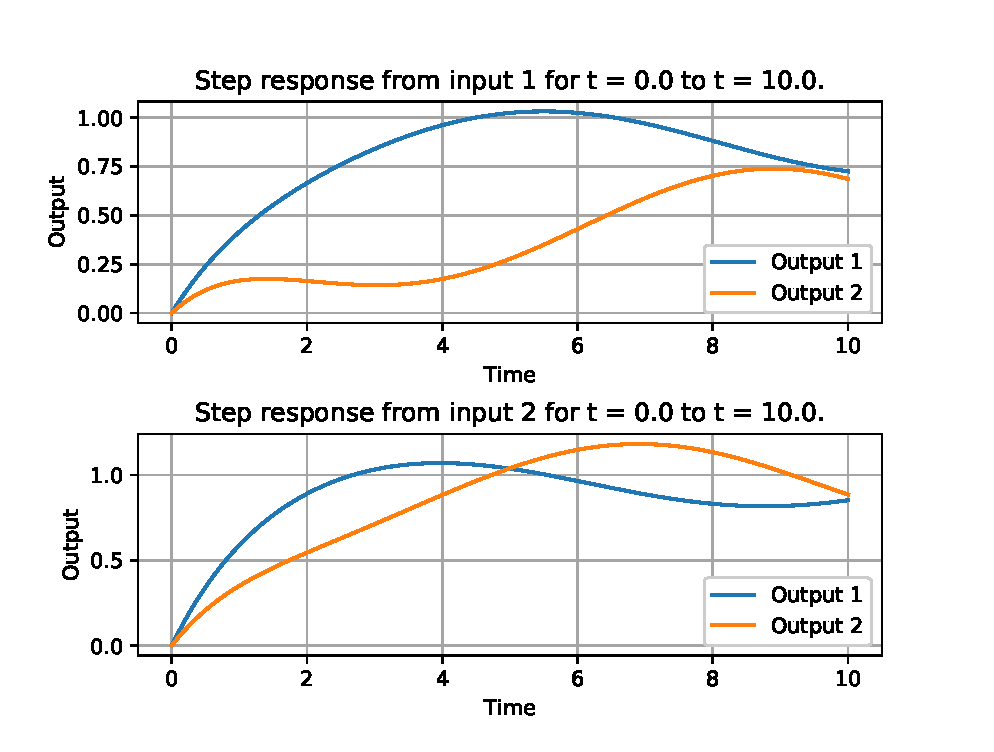
\includegraphics[scale=0.8]{cont_step}
	\caption{The response of all 3 output variables of a continuous dynamical system to step inputs on each of its 2 inputs.}
	\label{cont_step}
\end{figure}



\begin{figure}[H]
	\centering
		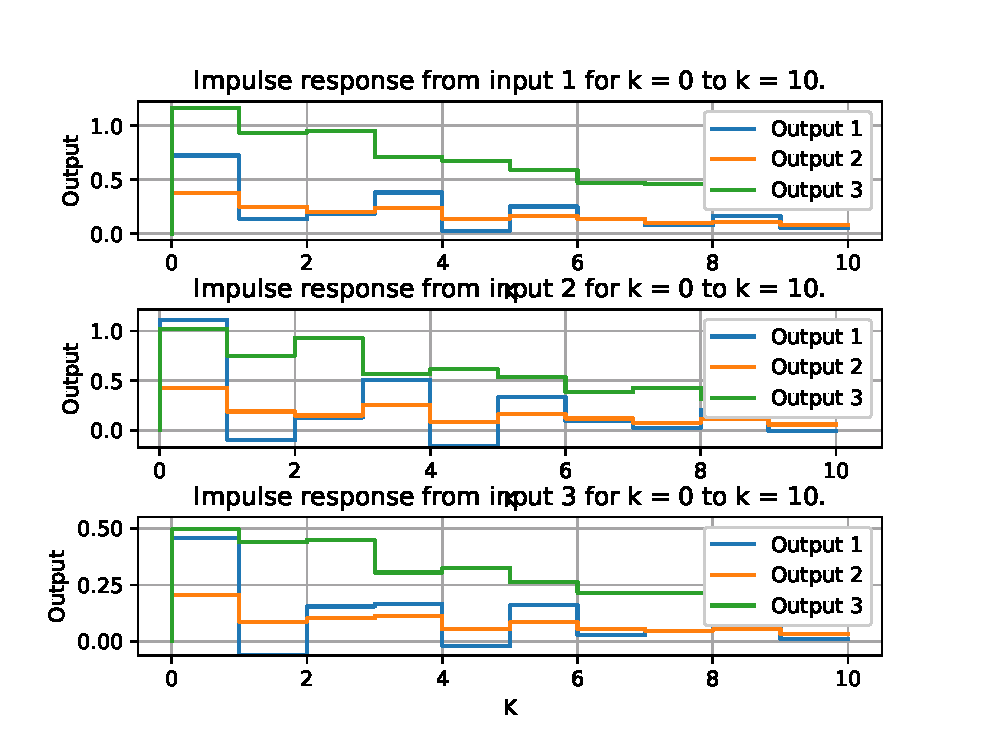
\includegraphics[scale=0.8]{disc_impulse}
	\caption{The response of all 3 output variables of a discrete dynamical system to step inputs on each of its 3 inputs.}
	\label{disc_impulse}
\end{figure}

\begin{figure}[H]
	\centering
		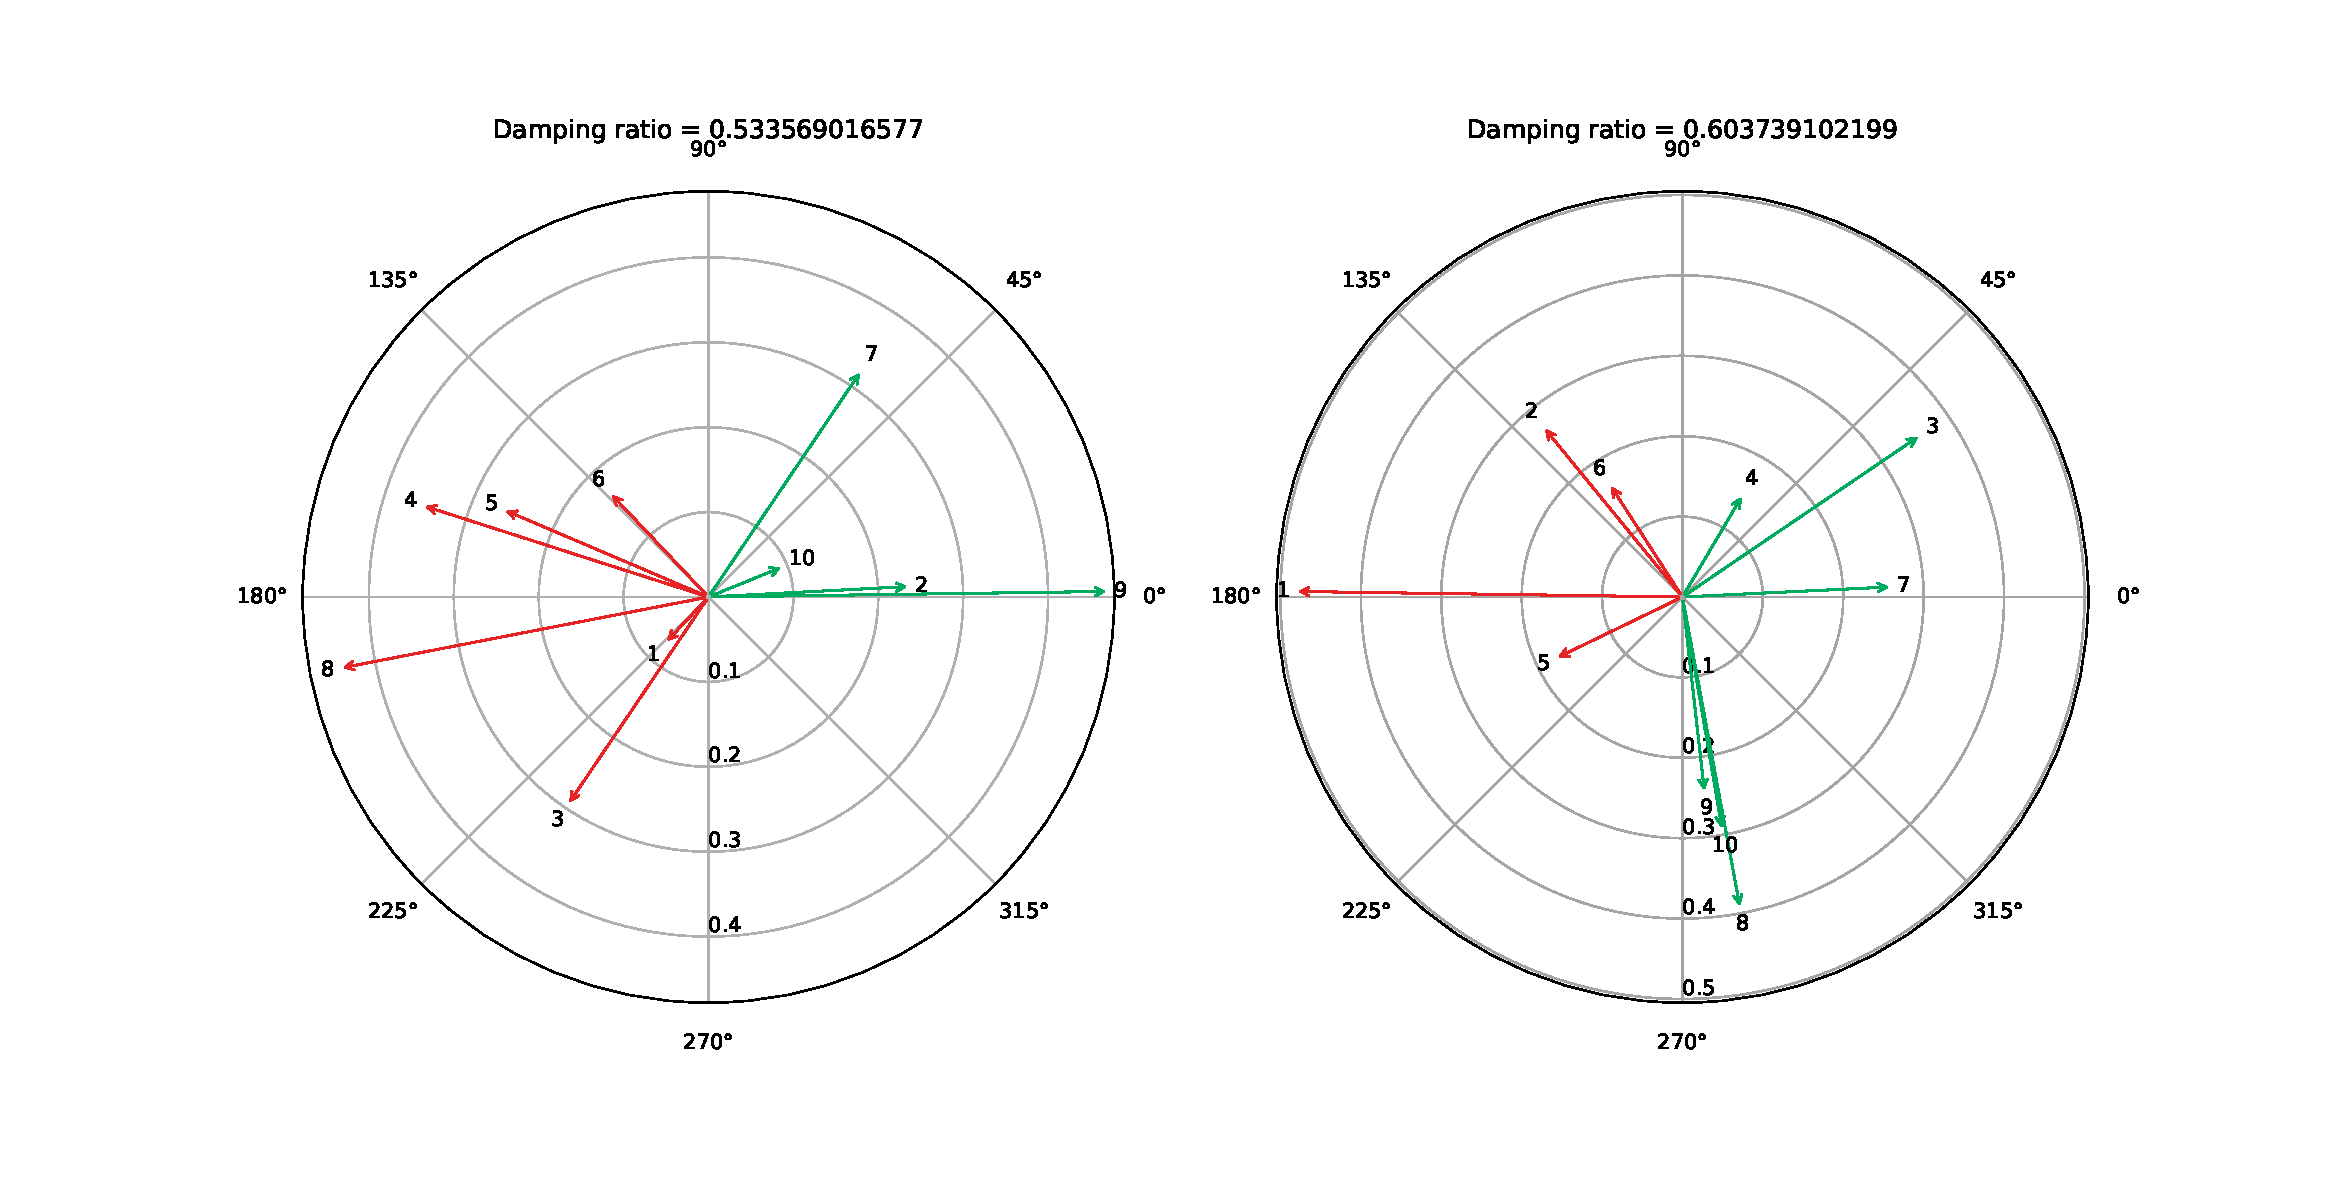
\includegraphics[scale=0.45]{compass}
	\caption{Compass plots showing the relative intensity and phase of the modes of a continuous dynamical system with greatest damping ratio. Mode 1 shows strong opposition between generators 4,5,8 and 2,9,10. Mode 2 shows strong opposition between generators 1 and 7.}
	\label{compass}
\end{figure}


\begin{figure}[H]
	\centering	
		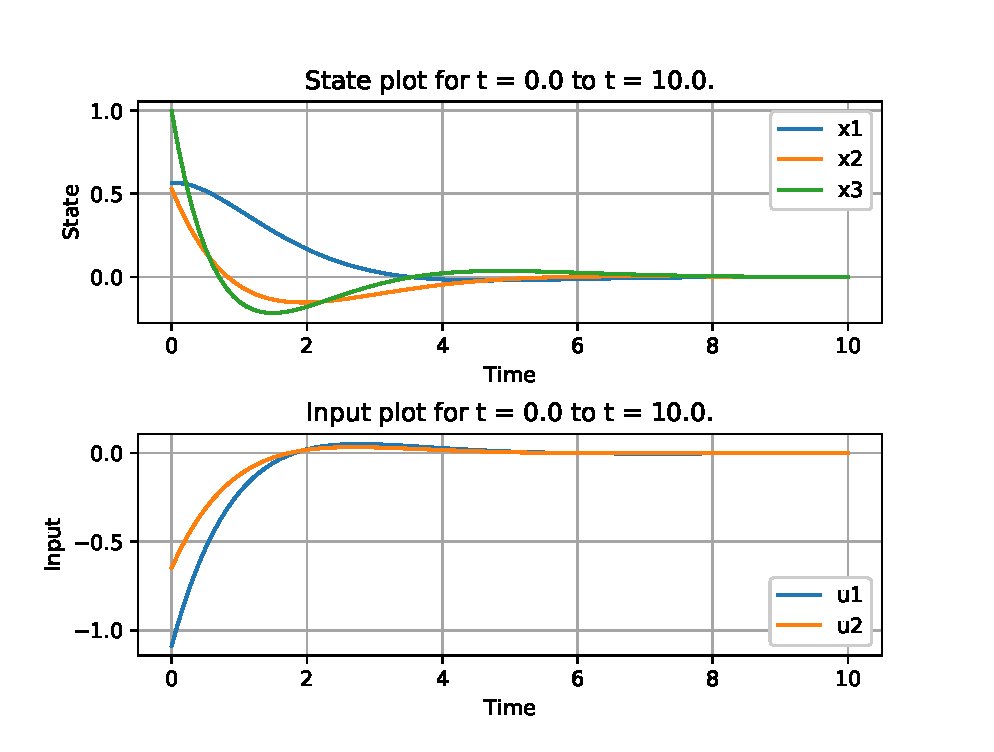
\includegraphics[scale=0.48]{inf_lqr_cont_4}
		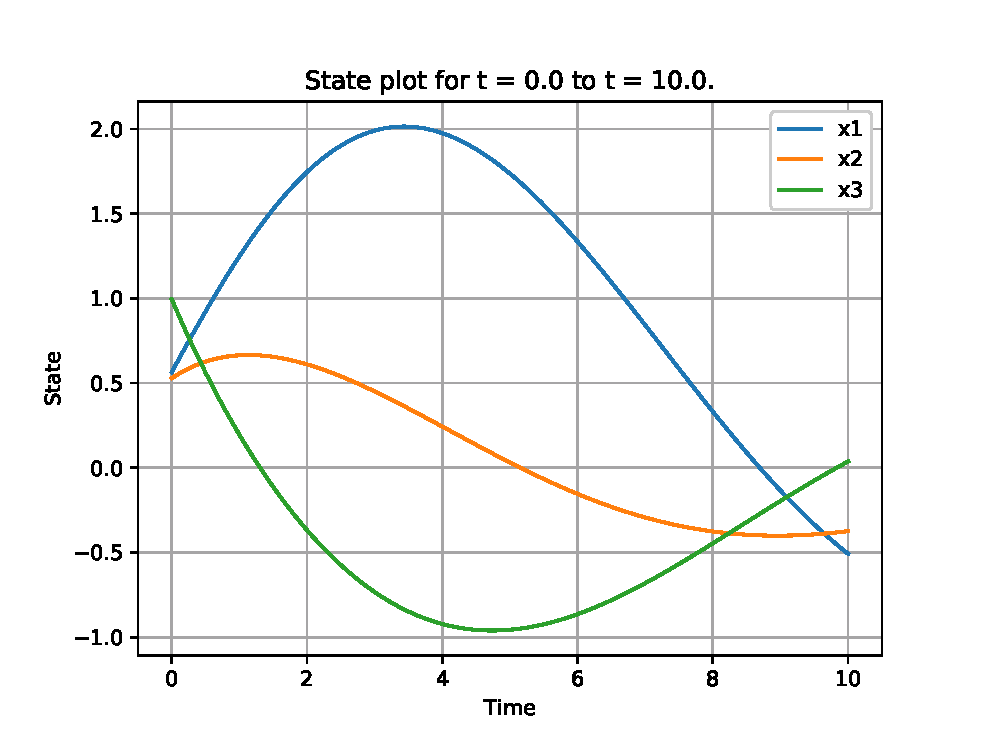
\includegraphics[scale=0.48]{cont_plot}

	\caption{Simulations derived from calculation of an infinite horizon LQR controller for a continuous dynamical system (\textit{left}) and the uncontrolled system (\textit{right}).}
	\label{inf_lqr_cont}
\end{figure}


\section*{Goals}
The overall goal of the project is to implement the System Level Approach for discrete controller synthesis and integrate it into the existing toolbox.

The System Level Synthesis (SLS) problem is formulated by considering the closed loop from state disturbances to the state and input variables and enforcing a finite horizon impulse response,
\begin{equation*}
\begin{bmatrix}
         x \\
         u \\
        \end{bmatrix}
=
\begin{bmatrix}
         R \\
         M \\
        \end{bmatrix}
\delta x
\end{equation*}

An optimization problem can then be formed to find the sets of matrices $R$ and $M$,

\begin{align*}
&\min \, \vert\vert C_{1}R+  D_{12}M\vert\vert_{\mathcal{H}_2} \\
\text{s.t.} \quad &\left[zI-A\, -B_{2} \right]
\begin{bmatrix}
	R \\
	M \\
\end{bmatrix}
 = I \\
&R,M \in \frac{1}{z}\mathcal{R H}_{\infty} \\ 
&R,M \in \mathcal{L}, \,\mathcal{F}_T, \,\mathcal{S} \\
\end{align*}

where $\mathcal{L}$ is the localizability constraint, $\mathcal{F}_T$ is the finite impulse response and $\mathcal{S}$ is the system level constraint. $\mathcal{RH}_{\infty}$ is the set of real rational proper transfer matrices.

\bibliographystyle{utphys}
\bibliography{first_interim_bib}


\end{document}